\documentclass{beamer}
\usetheme{Bruno}

\title[IoT for Rural Aqueducts using MBSE]{Towards a Modular IoT System Architecture for Rural Aqueducts using Model-Based Systems Engineering}
\author[Laboratorio Delta]{Anthony José Arguedas-Rodríguez \and María José Angulo-Campos \and Juan José Montero-Jiménez \and Juan José Rojas-Hernández}
\date{2025 IEEE International Symposium on Systems Engineering}

\begin{document}

\begin{frame}
    % Title in large font
    \begin{center}
        % Access the title variable
        {\LARGE \textbf{\inserttitle}} \\
        \vspace{0.5cm}
        {\insertauthor} \\
        \vspace{0.25cm}
        {\small \textbf{Laboratorio Delta, Costa Rica Institute of Technology}} \\
        \vspace{0.5cm}
        {\insertdate}
    \end{center}
\end{frame}

\begin{frame}
    \frametitle{Contents}
    \begin{itemize}
        \item IoT Systems in Rural Aqueducts Context
        \item ARCADIA Model-Based Systems Engineering (MBSE) Methodology
        \item Operational Need Analysis: What Rural Aqueducts Need to Accomplish
        \item System Need Analysis: What IoT Systems Must Accomplish for Rural Aqueducts
        \item A Generic and Modular IoT Logical Architecture
        \item Physical Architecture: A Case Study of ASADA Paso Ancho, Costa Rica
        \item Conclusions and Future Work
    \end{itemize}
\end{frame}

\begin{frame}
    \frametitle{IoT Systems in Rural Aqueducts Context}
    \framesubtitle{Capability gaps in rural aqueducts and the role of technology transfer initiatives}

    \begin{figure}
        \centering
        
\includegraphics[width=\textwidth]{images/before_and_after_iot.png}
        \caption{Comparison of rural aqueducts with and without IoT systems, with technology transfer initiatives as contributors to IoT implementation.}
    \end{figure}
\end{frame}

\begin{frame}
    \frametitle{The ARCADIA MBSE Methodology}
    \framesubtitle{Need Understanding}

    \begin{figure}
        \centering
        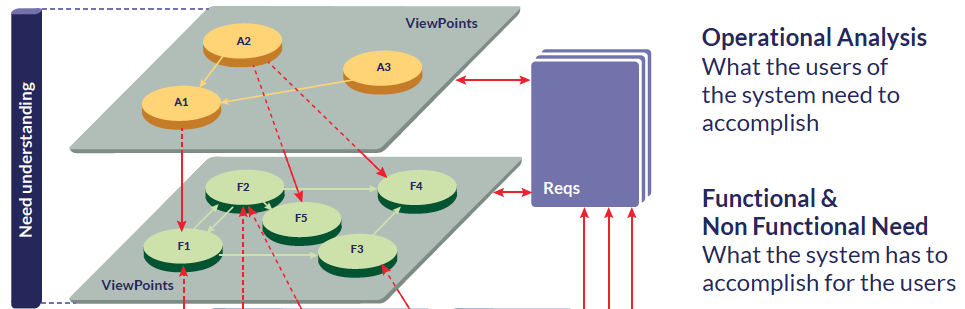
\includegraphics[width=\textwidth]{images/phases_arcadia_1.png}
        \caption{Need Understanding phases of the ARCADIA Model-Based Systems Engineering Methodology \cite{Arcadia_phases}.}
    \end{figure}
\end{frame}

\begin{frame}
    \frametitle{The ARCADIA MBSE Methodology}
    \framesubtitle{Solution Architectural Design}

    \begin{figure}
        \centering
        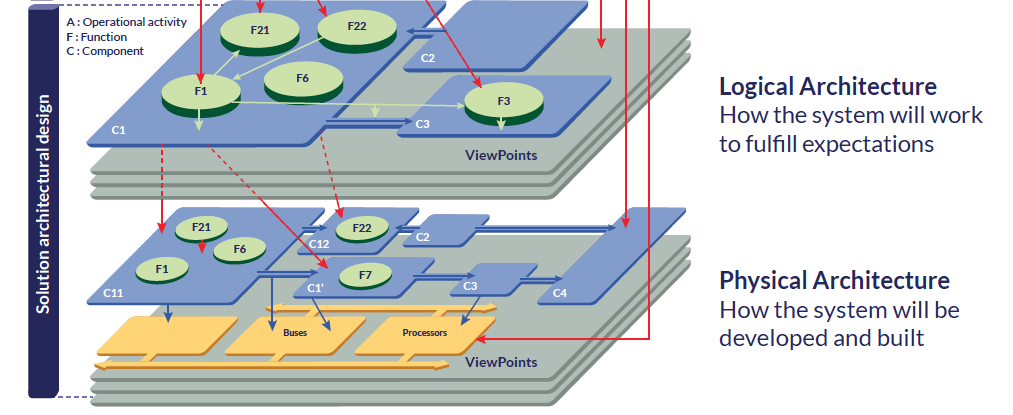
\includegraphics[width=\textwidth]{images/phases_arcadia_2.png}
        \caption{Solution Architectural Design phases of the ARCADIA Model-Based Systems Engineering Methodology \cite{Arcadia_phases}.}
    \end{figure}
\end{frame}

\begin{frame}
    \frametitle{Extracting Generic Needs and Desires about IoT Systems in Rural Aqueducts}

    \begin{figure}
        \centering
        
\includegraphics[width=\textwidth]{images/bertopic.png}
        \caption{Process of extracting generic needs and desires about IoT systems in rural aqueducts from published literature.}
    \end{figure}
\end{frame}

\begin{frame}
    \frametitle{Operational Need Analysis}
    \framesubtitle{Operational Capabilities 1: Provide high-quality water, 2: Comply with water quality standards and 4: Share data with external entities}

    \begin{figure}
        \centering
        \includegraphics[width=\textwidth]{images/opcap1.jpg}
        \caption{Operational Need Analysis for rural aqueducts, reduced to the activities involved in Capabilities 1, 2 and 4.}
    \end{figure}
\end{frame}

\begin{frame}
    \frametitle{Operational Need Analysis}
    \framesubtitle{Operational Capability 3: Mitigate water loss}

    \begin{figure}
        \centering
        
\includegraphics[width=\textwidth]{images/opcap3.jpg}
        \caption{Operational Need Analysis for rural aqueducts, reduced to the activities involved in Capability 3.}
    \end{figure}
\end{frame}

%\begin{frame}
%    \frametitle{System Need Analysis}
%    \framesubtitle{System Capabilities 1 (Provide water quality data), 5 (Share data with external entities)}
%
%    \begin{figure}
%        \centering
%        \includegraphics[width=\textwidth]{images/syscap1.jpg}
%        \caption{System Need Analysis for IoT systems in rural aqueducts, reduced to the activities involved in Capabilities 1 and 5.}
%    \end{figure}
%\end{frame}

\begin{frame}
    \frametitle{References}
    \bibliographystyle{IEEEtran}
    \bibliography{refs}
\end{frame}

\end{document}